\chapter{レンズによる提案手法の検討}
\thispagestyle{empty}
\label{chap4}
\graphicspath{{chap4/figure/}}
\minitoc

\newpage
%%%%%%%%%%%%%%%%%%%%%%%%%%%%%%%%%%%%%%%%%%%%%%%%%%%%%%%%%%%%%%%%%%%%%%%%%%%%%


% ================================================== %
% section
% ================================================== %
\section{諸言}
\label{chap4_introduction}


\clearpage
% ================================================== %
% section
% ================================================== %
\newpage

\section{実験の構成および設計パラメータ}
3章で提案された手法について、ミラーの測定実験を行う前に、レンズを用いた実験を行い、手法の実現可能性について検討する。
波面計測の対象となるミラー下流端開口の集光波面を再現できれば、手法の検討を行うことができる。
これは、平行光に対して輪帯状の開口を入れ、さらにレンズによって集光することで、輪帯状の集光球面波を作ることができ擬似的にミラー下流端面を再現することができる。

レンズによる選定に際して、本来の測定対象であるWolterミラーと同様の系を構成するべきであるが、入手性の問題からここでは口径は異なるがNAがほぼ等しいレンズを用いて実験を行う。
用いたレンズのパラメータは表\ref{tb:focusing_lens_params}に示す通りである。

\begin{table}[h]
\begin{center}
  \begin{tabular}{|c|c|} \hline
    パラメータ & 値 \\ \hline
    直径 & 30.0 mm  \\
    焦点距離 & 1000.000 mm \\
    設計波長 & 541.6 nm \\ \hline
  \end{tabular}
  \caption{レンズの設計パラメータ}
  \label{tb:focusing_lens_params}
\end{center}
\end{table}

これに合わせて、輪帯開口およびピンホールを図\ref{fig:lens_pinhole_ring_aperture}の用に設計した。
輪帯幅を変えて実験を行うため、図\ref{fig:lens_ring_aperture}における$A$を表\ref{tb:lens_ring_aperture_inner_diameter}のように3通り用意した。

\begin{figure}[!ht]
\centering

\subfloat[輪帯アパーチャ]{
    \centering
    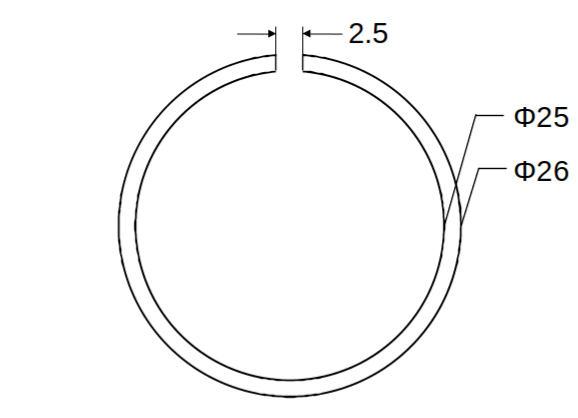
\includegraphics[scale=0.5]{ring_aperture.png}
    \label{fig:lens_ring_aperture}
}
\subfloat[ピンホール]{
    \centering
    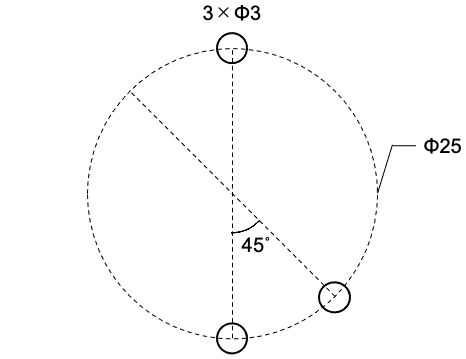
\includegraphics[scale=0.5]{pinhole_arrangement.png}
    \label{fig:lens_pinhole_arrangement}
}
\caption[]{設計図面}
\label{fig:lens_pinhole_ring_aperture}
\end{figure}

\begin{table}[h]
\begin{center}
  \begin{tabular}{|c|c|l|} \hline
    番号 & A & 輪帯幅 \\ \hline
    1 & 25 mm & 1 mm \\
    2 & 25.5 mm & 0.5 mm \\
    3 & 25.75 mm & 0.25 mm \\ \hline
  \end{tabular}
  \caption{輪帯アパーチャ内円の直径}
  \label{tb:lens_ring_aperture_inner_diameter}
\end{center}
\end{table}

レーザーでの加工の都合上、もっとも細い輪帯幅0.25 mmのものについてはレーザーを輪帯状に1度走査するという方法を取ったため、設計寸法は参考値となる。

\clearpage
% ================================================== %
% section
% ================================================== %
\newpage


\section{疎条件を利用した位相回復の結果}
回復計算に用いたパラメータは以下の通りである。

回復計算が収束しなかった。


\clearpage
% ================================================== %
% section
% ================================================== %
\newpage

\section{下流端走査によるタイコグラフィの結果}


\clearpage
% ================================================== %
% section
% ================================================== %
\newpage

\section{結論}
\label{chap4_conclusion}


%%%%%%%%%%%%%%%%%%%%%%%%%%%%%%%%%%%%%%%%%%%%%%%%%%%%%%%%%%%%%%%%%%%%%%%%%%%%%
%%% Local Variables:
%%% mode: katex
%%% TeX-master: "../thesis"
%%% End:
